%%%%%%%%%%%%%%%%%%%%%%%%%%%%%%%%%%%%%%%%%%%%%%%%%%%%%%%%%%%%%%%%%%%%%%%%%%%%%%%%
% operation.tex: Chapter on Detector Operation and Performance:
%%%%%%%%%%%%%%%%%%%%%%%%%%%%%%%%%%%%%%%%%%%%%%%%%%%%%%%%%%%%%%%%%%%%%%%%%%%%%%%%
\chapter{Detector In-Flight Performance}
\label{operation_chapter}
%%%%%%%%%%%%%%%%%%%%%%%%%%%%%%%%%%%%%%%%%%%%%%%%%%%%%%%%%%%%%%%%%%%%%%%%%%%%%%%%

We discuss the detector yield, Section~\ref{sec:yield}, and the detectors' measured radiative loads, Section~\ref{sec:radiative_load}.
In section~\ref{sec:flight_noise_performance}, using the dark characterization measurements, the measured radiative load, the electrical bias parameters, and the \ac{DfMUX} transfer functions, we predict the instrument sensitivity in \ac{NEP}. 
We report the noise performance of each detector by comparing its expected \ac{NEP} to the median of its measured \ac{NEP} over all portions of the \ac{EBEX} flight for which it had valid data. 


%%%%%%%%%%%%%%%%%%%%%%%%%%%%%%%%%%%%%%%%%%%%%%%%%%%%%%%%%%%%%%%%%%%%%%%%%%%%%%%%
% Detector Yield 
%%%%%%%%%%%%%%%%%%%%%%%%%%%%%%%%%%%%%%%%%%%%%%%%%%%%%%%%%%%%%%%%%%%%%%%%%%%%%%%%
\section{Detector Yield}
\label{sec:yield}
%%%%%%%%%%%%%%%%%%%%%%%%%%%%%%%%%%%%%%%%%%%%%%%%%%%%%%%%%%%%%%%%%%%%%%%%%%%%%%%%

\begin{table}[ht!]
\begin{center}
\begin{tabular}{l|c|c|c|c}
  & 150~GHz & 250~GHz & 410~GHz & Total \\
\hline Total number of bolometers on wafers & 1120 & 560 & 280 & 1960 \\
\hline Able to read out with \ac{EBEX} electronics & 992 & 496 & 254 & 1742 \\
\hline Passed warm electrical \& visual inspections & 908 & 455 & 232 & 1595 \\
\hline Resistor \& dark \ac{SQUID} channels excluded & 861 & 447 & 213 & 1521 \\
\hline Detectors appearing in .8~K network analysis & 805 & 430 & 187 & 1422 \\
\hline Detectors after SQUID failures removed & 773 & 414 & 155 & 1342 \\
\hline Detectors after noise polluters removed & 676 & 371 & 133 & 1180 \\
\hline Detectors with successful flight IV curves & 504 & 342 & 109 & 955 \\
% not including eccosorb/dark 492 & 317 & 92 & \
\hline
\end{tabular}
\end{center}
\caption[Detector yield]{The detector yield broken down by observation frequency band, 150, 250, and 410~GHz, as well as the sum. Each row of the table accounts for detector loss.}
\label{yield_table}
\end{table}

\TAB\ref{yield_table} provides an accounting of \ac{EBEX} detector yield as a function of observation frequency band, as well as the total for the experiment.
Each silicon wafer, regardless of observation frequency band, had 140 bolometers and one fabrication alignment mark. %for the curious/pedantic
The 150 and 250~GHz wafers were coupled to \ac{LC} boards around the perimeter of the focal plane. These edge \ac{LC} boards each had 125 readout channels. Because of the alignment mark replacing one bolometer, 124 readout channels were connected to bolometers.  
The 410~GHz wafers were in the center of each focal plane and had central \ac{LC} boards offset from the focal plane, in the space just behind the wafer. The central \ac{LC} boards each had 128 readout channels. Again, because of the alignment mark, 127 readout channels were connected to bolometers. %(because of the alignment mark). 
The first two rows of \TAB\ref{yield_table} give the total number of bolometers flown and the total number of bolometers the electronics were capable of reading out. 

At room temperature, the wafers were inspected visually and each bolometer was tested for electrical continuity. 
The visual inspection was done under a microscope and, for example, sometimes revealed incomplete etching evidenced by a column of silicon from the spiderweb to the silicon backing wafer. 
This was noted as a thermal short and such a detector was not electrically biased. 
For the electrical inspection, we measured the resistance by either probing directly across the wafer bond pads or by probing the leads on the \ac{LC} boards. 
The first method was done in the fabrication clean room and the second method was done after the wafer had been shipped, mounted, and wirebonded to its \ac{LC} board. 
The resistance reading was dominated by the room temperature resistance of the niobium leads. 
The electrical inspection could not identify a short across the \ac{TES} because the typical room temperature resistance of the \ac{TES} was a few ohms, much less than the tens of kiloohms of the niobium leads. 
The electrical inspection did, however, identify which \ac{TES} or leads did not make a complete electrical connection, i.e. were open. 
The warm visual and electrical inspection provided an upper limit of the wafer's yield because the open and thermally shorted detectors were guaranteed not to work, third row of \TAB\ref{yield_table}. 

For flight, each wafer had two bolometers replaced by one ohm resistors near the \ac{LC} board bond pads. 
These two channels were dedicated to monitoring read out electronic noise up to the \ac{LC} board, one channel at a low bias frequency and the other channel at a high bias frequency. 
Three \ac{SQUID}s were not attached to bolometer combs due to opens in the microstrips. These combs were modified to monitor read out electronic noise up to the \ac{SQUID}, \TAB\ref{yield_table} row 4. 

Upon cooling the wafer, there were wired detector channels which had shown a reasonable room temperature resistance but did not appear in the network analysis, \TAB\ref{yield_table} row 5. 
Five \ac{SQUID}s failed to operate during flight, \TAB\ref{yield_table} row 6. 
Once a wafer was characterized in a dark cryostat, the detectors which degraded the noise performance of their entire comb were identified and their wirebonds were removed, \TAB\ref{yield_table}, row 7. 
%%Occasionally, upon cooling a wafer a second time, additional detectors go missing from the network analysis. (And some detectors re-appear ... presumably due to poor quality wirebond connections.) See \TAB\ref{yield_table}, line "Survived \ac{EBEX} cooldown and plucking." \comred{remove word plucking and remove bad actor, replace with more clear description. no need to mention reappearances since they seldom happen and we only have conjectures as to why?}

After \ac{EBEX} was launched and reached its float altitude, IV curves were performed and the total number of successful curves is reported in \TAB\ref{yield_table}, line 8. 
The losses between row 7 and row 8 were due to detectors being saturated or failing to transition. 

%(though typically they also failed to turn around during the characterization measurements, the loss isn't counted until flight because there was some hope they might work) or the IV curve exhibiting strange behaviour (e.g. a jump in the current reading). \comred{ben showed pv curve, but not iv curve. maybe just call it a pv curve and refer to detector fab section? NO. with reorganization, first mention of iv/pv curve comes after this table ??}
%
%

%%%%%%%%%%%%%%%%%%%%%%%%%%%%%%%%%%%%%%%%%%%%%%%%%%%%%%%%%%%%%%%%%%%%%%%%%%%%%%}}}


%%%%%%%%%%%%%%%%%%%%%%%%%%%%%%%%%%%%%%%%%%%%%%%%%%%%%%%%%%%%%%%%%%%%%%%%%%%%%%%%
% Measured Radiative Loads 
%%%%%%%%%%%%%%%%%%%%%%%%%%%%%%%%%%%%%%%%%%%%%%%%%%%%%%%%%%%%%%%%%%%%%%%%%%%%%%%%
\section{Radiative Load}
\label{sec:radiative_load}
%%%%%%%%%%%%%%%%%%%%%%%%%%%%%%%%%%%%%%%%%%%%%%%%%%%%%%%%%%%%%%%%%%%%%%%%%%%%%%%%

%\textcolor{red}{Need to go write the thermal conductance measurement section. } 
%\textcolor{red}{remove shoulds below. be quantitative (somewhere) about what it is and the effect this has on the powers we measure/report.}

%The following was already mentioned in bolo theory. 
%The steady state power flow from the bolometer to the bath is a combination of the electrical bias power and the power absorbed from the radiative load,
%\be
%P_{total} = P_{electrical} + P_{radiative}
%\label{eq:total_power}
%\ee
The IV curve measurements, described in Section~\ref{sec:thermal_conductance}, provided the electrical power required to hold the detector in the negative electrothermal feedback regime. 
In the dark test cryostats, ideally, the radiative load was negligible and so the only power on the detectors was the electrical bias power. 
That is, for the dark test cryostat IV curve measurements, Equation~\ref{eq:pin} became
\be
P_{total} = P_{elec} + \cancel{P_{rad}},
\label{eq:total_power_dark}
\ee
We measured $P_{elec}$ dark and that was $P_{total}$, the total power necessary to hold the detector in the negative electrothermal feedback regime. 

Once \ac{EBEX} reached float altitude and the thick cryostat window was rolled back, IV curves were performed for all detectors. 
From these IV curves, we measured the electrical power required at float, with the radiative load present, to hold the detector in the negative electrothermal feedback regime. 
The difference in the two powers measured, in the dark cryostat and open to light at float, gave each detector's measured radiative load,
\be
P_{rad} = P_{elec}^{dark} - P_{elec}^{float},
\label{eq:radiative_load}
\ee
Figure~\ref{fig:dark_light_iv_curves} shows two PV curves for a 250~GHz detector dark in \ac{ETC} and open to light at float in \ac{EBEX}. 

\begin{figure}[htp]
\begin{center}
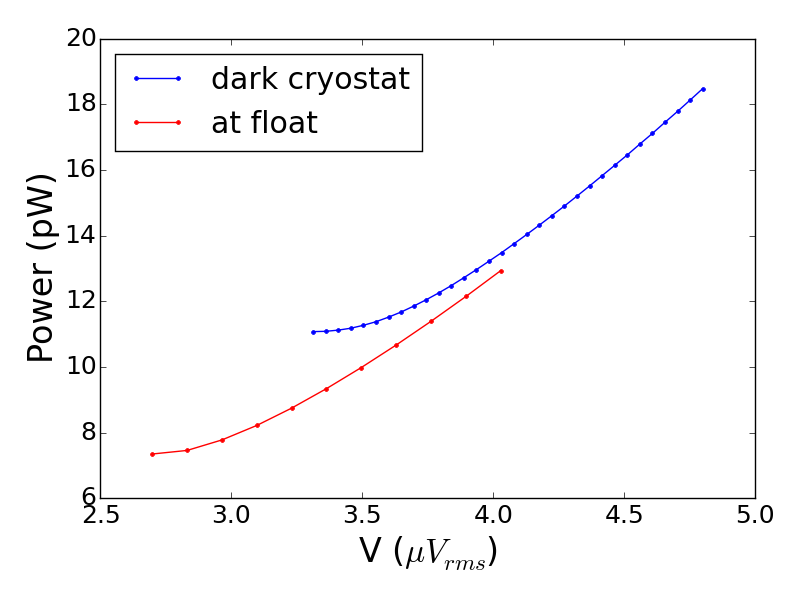
\includegraphics[height=2.5in]{figures/board64_wire3_ch06_pv_dark_and_float.png}
\caption[PV curves dark in test cryostat and open to light at float]{Electrical power as a function of bias voltage for a detector from a 250~GHz wafer, dark in \ac{ETC} (blue) and at float (red). At float, because of the radiative load, less electrical power was required to hold the detector in the negative electrothermal feedback regime. The difference in electrical powers, 4~pW, was the measured radiative load 
%\textcolor{red}{Is this the bolometer you want to showcase? (the same one used in EP2.) NO. PICK ONE FROM ETC, 250-23 ?}
\label{fig:dark_light_iv_curves} }
\end{center}
\end{figure}

%COME BACK HERE IF YOU HAVE TIME
%\textcolor{red}{Is it worth mentioning anywhere that we also did IV curves as a function of elevation and also after each fridge cycle?}

%KIND OF DID THIS IN CHARACTERIZATION SECTION
%\textcolor{red}{Do you want to say anything about how and why we dropped to 85\%? Can you make a quantitative statement about the level of uncertainty or systematic this introduces in $P_{sat}^{light}$}

%\textcolor{red}{You need to be clear about what was done for differing bath temperatures. Perhaps this is best addressed in the IV curve section.}



Figure~\ref{fig:radiative_load_histograms} has the distributions of the measured radiative loads from the first set of IV curves performed at float, broken down by observation frequency band. 
The measured radiative loads were Gaussian-shaped distributions. 
The Gaussian fits, of $3.6\pm 1.0, \, 5.3\pm 1.8$, and $4.9 \pm 1.4$~pW, agreed closely with the  medians and standard deviations of the distributions, $3.6\pm1.5, \, 5.3\pm1.8$, and $5.0\pm1.4$~pW, 
for 150, 250, and 410~GHz, respectively. 
There were 37, 9, and 0 detectors at 150, 250, and 410~GHz with negative measured loads. 
These non-physical measurements were not understood and not included in the radiative load distributions. 

The predicted radiative loads were generated by calculating the transmission, reflection, and absorption of each element in the detector's optical path \textcolor{red}{[EP2]}.  
%\ref{Zilic2014}.  NO! HE DOESN'T HAVE THE INFO IN THERE. BUT KEVIN DOES. BUT KEVIN HAD THE WRONG WINDOW THICKNESS. FORGET REFERENCING SINCE CAN'T REFERENCE SHAUL'S SPREADSHEET. 
Assuming detector efficiencies of 0.6, 0.5, and 0.4 at 150, 250, and 410~GHz, the predicted loads were 1.4, 3.7, and 4.7~pW, see Table~\ref{tab:target_gbar}.
At 250 and 410~GHz, these pre-flight predictions fall within one standard deviation of the measured radiative load. 
At 150~GHz, the detector efficiency would have to have been 150\% in order for the measurement to have matched the predicted load. 
This unphysical result tells us there was an excess load in the 150~GHz band. 
Assuming the detector efficiency was actually $\sim$80\%, as was measured in \ac{ETC}, Section~\ref{sec:optical_efficiency}, then the incident power on the 150~GHz bolometers was 4.5~pW, 2.1~pW in excess of the predicted incident power of 2.4~pW. 
%\textcolor{red}{Discuss the results of this measurement more? Is there anything else to say? Reference EP2?}

\begin{figure}[htp]
\begin{center}
%\begin{tabular}{cc}
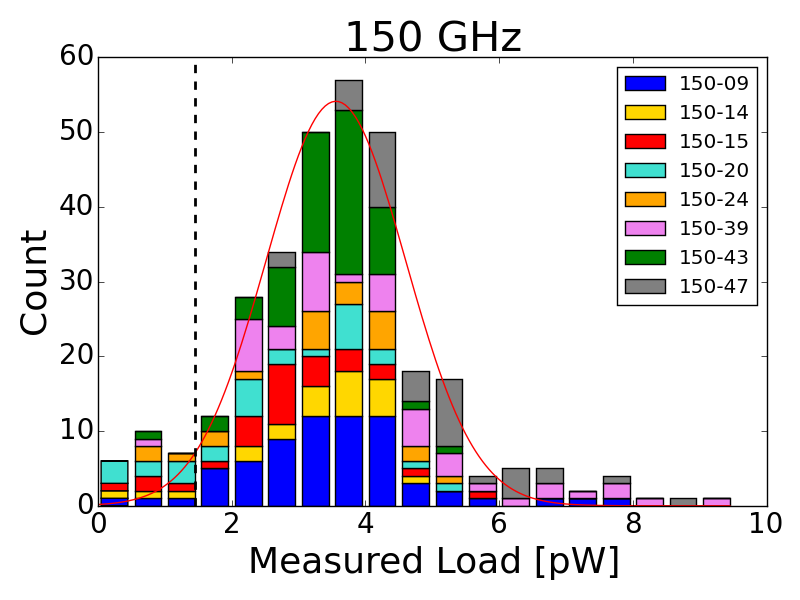
\includegraphics[width=0.32\columnwidth]{figures/thesis_150_radiative_load_hist.png}
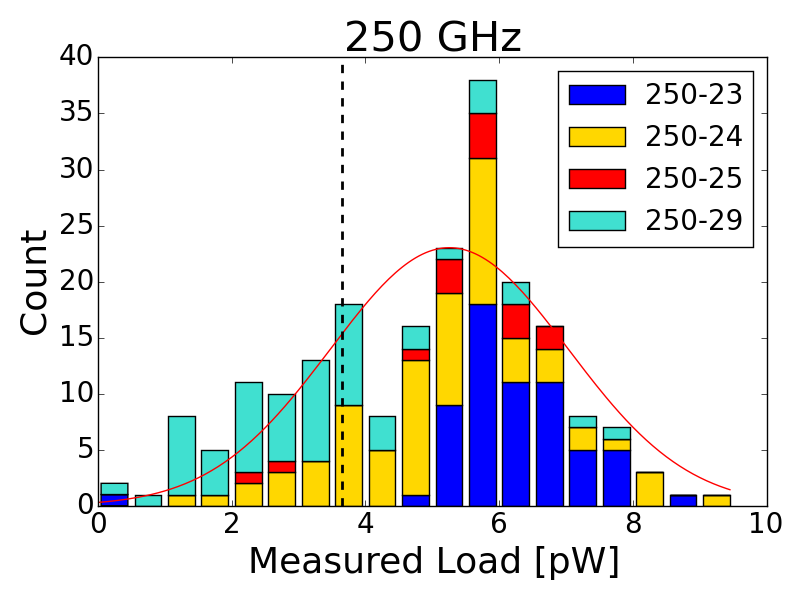
\includegraphics[width=0.32\columnwidth]{figures/thesis_250_radiative_load_hist.png}
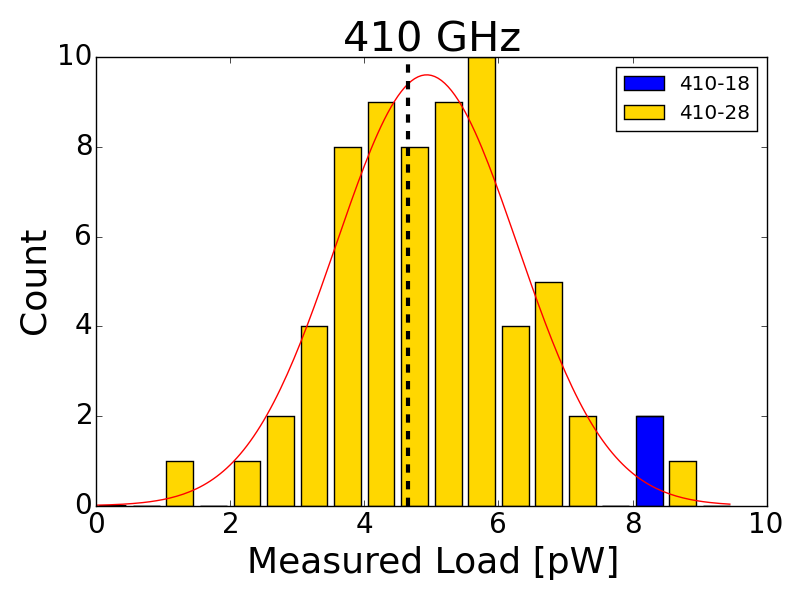
\includegraphics[width=0.32\columnwidth]{figures/thesis_410_radiative_load_hist.png}
%\end{tabular}
\caption[Radiative load histograms]{Histograms of the measured radiative load from the first detector tuning at float. 
The different colors represent different wafers.  
The thin red lines are the gaussian fits of $3.6\pm1.0, \, 5.3\pm1.8$, and $4.9\pm1.4$~pW for the 150, 250, and 410~GHz observation bands, respectively. 
The black dashed vertical lines are the pre-flight predicted loads of 1.4, 3.7, and 4.7~pW, assuming detector efficiencies of 0.6, 0.5, and 0.4, for 150, 250, and 410~GHz. 
\label{fig:radiative_load_histograms} }
\end{center}
\end{figure}


%COME BACK TO THIS IF YOU HAVE TIME
%\textcolor{red}{Do you want to mention the patterns of the wafers? Namely, calculate medians by wafer. Suspect you'll see the median measured by 250-23 is higher than that measured by 250-29 and 250-24 and 250-25 fall somewhere in between and the differences are non-negligible, i.e. more than one standard deviation away from each other?}

%%%%%%%%%%%%%%%%%%%%%%%%%%%%%%%%%%%%%%%%%%%%%%%%%%%%%%%%%%%%%%%%%%%%%%%%%%%%%%}}}



%%%%%%%%%%%%%%%%%%%%%%%%%%%%%%%%%%%%%%%%%%%%%%%%%%%%%%%%%%%%%%%%%%%%%%%%%%%%%%%%
% Detector Flight Performance 
%%%%%%%%%%%%%%%%%%%%%%%%%%%%%%%%%%%%%%%%%%%%%%%%%%%%%%%%%%%%%%%%%%%%%%%%%%%%%%%%
\section{In-Flight Noise Performance}
\label{sec:flight_noise_performance}
%%%%%%%%%%%%%%%%%%%%%%%%%%%%%%%%%%%%%%%%%%%%%%%%%%%%%%%%%%%%%%%%%%%%%%%%%%%%%%%%

% you already said this at the beginning.
%The predicted \ac{NEP} is calculated using measurements of detector parameters and radiative load. 
%The measured \ac{NEP} is calculated from flight data. 
The noise performance is assessed by comparing the predicted \ac{NEP} to the measured ac{NEP}. 
We look at the noise of the dark \ac{SQUID}s, the resistor channels, the bolometers overbiased while the stage is cold, and the bolometers dropped into their superconducting transition state. 

%%%%%%%%%%%%%%%%%%%%%%%%%%%%%%%%%%%%%%%%%%%%%%%%%%%%%%%%%%%%%%%%%%%%%%%%%%%%%%%%
\subsection{NEP unit conversions}
\label{sec:nep_units}
%%%%%%%%%%%%%%%%%%%%%%%%%%%%%%%%%%%%%%%%%%%%%%%%%%%%%%%%%%%%%%%%%%%%%%%%%%%%%%%%

There are four units we use when measuring the detector \ac{NEP}: \ac{DfMUX} \ac{ADC} counts, Amps, Watts at the detector, and Watts on the sky. 
The raw timestreams from the \ac{DfMUX} boards are recorded in \ac{ADC} counts. 
The predictions for the current noise terms of the \ac{NEP}, Johnson and readout, are naturally in units of Amps.
The predictions for the power noise terms of the \ac{NEP}, photon and phonon, are naturally in units of Watts at the detector. 
To convert to units of power on the sky, we can either use each detector's calibration map of RCW38 or the measured end-to-end instrument efficiency, 
\be
\varepsilon = \frac{\text{power absorbed by detector}}{\text{incident sky power}}
\label{eq:eff_ratio}
\ee
Table~\ref{tab:psd_table} provides the conversion applied to each noise term in order to report in the units of the leftmost column. 

\begin{table}[htp]
\begin{center}
\begin{tabular}{|c|c|c|c|}
\hline Units & Timestream & Photon and Phonon & Johnson and Readout \\ 
\hline ct & $\big( \frac{\textbf{ct}^2}{\textbf{Hz}} \big)$ & $\big( \frac{W_{bolo}^2}{Hz} \big)   \big( S_I \big) ^2 \big( \frac{\text{ct}}{A} \big) ^2$ & $\big( \frac{A^2}{Hz} \big) \big( \frac{\text{ct}}{A} \big) ^2 $ \\ 
\hline A & $\big( \frac{\text{ct}^2}{\text{Hz}} \big) \big( \frac{A}{\text{ct}} \big) ^2 $ & $\big( \frac{W_{bolo}^2}{Hz} \big) \big( S_I \big) ^2$ & $\big( \frac{\textbf{A}^2}{\textbf{Hz}} \big)$ \\ 
\hline $W_{bolo}$ & $\big( \frac{\text{ct}^2}{\text{Hz}} \big) \big( \frac{A}{\text{ct}} \big) ^2 \big( \frac{1}{S_I} \big) ^2$ & $\big( \frac{\textbf{W}_{bolo}^2}{\textbf{Hz}} \big)$ & $\big( \frac{A^2}{Hz} \big) \big( \frac{1}{S_I} \big) ^2$ \\ 
\hline $W_{sky}$ &  $\big( \frac{\text{cts}^2}{\text{Hz}} \big) \big( \frac{W_{sky}}{\text{ct}} \big) ^2$ & $\big( \frac{W_{bolo}^2}{Hz} \big) \big( S_I \big) ^2 \big( \frac{\text{ct}}{\text{A}} \big) ^2 \big( \frac{W_{sky}}{\text{ct}} \big) ^2$ & $\big( \frac{A^2}{Hz} \big) \big( \frac{\text{ct}}{A} \big) ^2 \big( \frac{W_{sky}}{\text{ct}} \big) ^2$ \\ 
\hline $W_{sky}$ & $\big( \frac{\text{cts}^2}{\text{Hz}} \big) \big( \frac{A}{\text{ct}} \big) ^2 \big( \frac{1}{S_I} \big) ^2 \big( \frac{1}{\varepsilon} \big) ^2$ & $\big( \frac{W^2}{Hz} \big)  \big( \frac{1}{\varepsilon} \big) ^2$ &  $\big( \frac{A^2}{Hz} \big) \big( \frac{1}{S_I} \big) ^2 \big( \frac{1}{\varepsilon} \big) ^2 $ \\
\hline
\end{tabular}
\end{center}
\caption[Unit conversions for noise equivalent power]{\ac{PSD} unit conversions used to get all noise terms in the same units. ct is a \ac{DfMUX} \ac{ADC} count, $W_{bolo}$ is power absorbed by the detector, $S_{I}$ is the detector current responsivity, $A$ is current though the \ac{SQUID}, $W_{sky}$ is power incident from the sky, and $\varepsilon$ is the end-to-end instrument optical efficiency. %incident upon the instrument? 
}
\label{tab:psd_table}
\end{table}


%%%%%%%%%%%%%%%%%%%%%%%%%%%%%%%%%%%%%%%%%%%%%%%%%%%%%%%%%%%%%%%%%%%%%%%%%%%%%%%%
\subsection{Procedure}
\label{sec:flight_procedure}
%%%%%%%%%%%%%%%%%%%%%%%%%%%%%%%%%%%%%%%%%%%%%%%%%%%%%%%%%%%%%%%%%%%%%%%%%%%%%%%%

%attempting to explain method for measuring noise
%1. How did you get wnl?
%2. what does it mean to have valid data?
%3. how many detectors had valid data? what fraction of their total data was valid?


As was done for the \ac{ETC} noise measurements reported in Section~\ref{sec:dark_noise}, the data was broken up into chunks of $\sim$3 minutes (172~seconds),
a gradient and offset were subtracted, a Hann window applied, and the \ac{PSD} was calculated. 
The \ac{WNL} was defined as the square root of the average of the \ac{PSD} from 3.9 to 4.4~Hz. 
This is a much narrower band than was used in the dark \ac{ETC} measurements. 
It was chosen because part of our signal of interest resided there, in one of the polarization frequency sidebands of 4*$f_{HWP}$~=~4*1.235~Hz~=~4.94~Hz. 
%This was a sideband safely away from the 4f signal. 
%the half-wave plate synchronous signal at

The following overbiased and in-transition noise analysis looked at the bolometers wired to \ac{BRO}s 2, 3, and 4. 
With the exception of the very first time the bolometers were dropped into their transitions at float and the subsequent half hour of observation, \ac{BRO}1 was turned off. 
This was in order to conserve bolometer crate power.
The bolometer crate batteries were not charged to their capacity because the gondola motor controller overheated and so the solar panels, responsible for charging the batteries, were not facing the sun as often as was planned. 
The cost to the overall data acquisition was small because \ac{BRO}1 happened to be wired to three wafers of bolometers which were largely saturated at float. 

Bolometer data, for purposes of noise analysis, were flagged if the detector was saturated, there were signals from cosmic ray absorption, there were \ac{SQUID} DC level jumps, the bolometer went superconducting, the \ac{HWP} synchronous signal subtraction failed, the \ac{HWP} motor was ramping on or off, the cryostat was stepping elevation, or the internal-to-the-cryostat calibrator was on. 
Flagged data was replaced by white noise realizations. 
In order for a chunk of data to be included in the noise analysis, we required no more than 10\% of the data be flagged. 
Of the 941 bolometers in \ac{BRO}2-4, 460 had data which passed the valid criteria. 
%IF YOU HAVE TIME, COME BACK HERE AND EXPLAIN WHERE YOU LOST THE DATA. ESPECIALLY BE ABLE TO SAY WHERE THE MAJORITY OF IT WAS (ASSUMING THERE WAS A MAJORITY LOST TO SOMETHING, E.G. SATURATION)

%SOME OF THIS SHOULD HAVE ALREADY BEEN MENTIONED IN BOLOMETER THEORY AND IN THE DARK NOISE MEASUREMENT SECTION. ALSO, IT'S OUT OF PLACE HERE.
%THE FOLLOWING IS ALREADY SPELLED OUT IN THE BOLO THEORY SECTION
%Responsivity is
%\be
%S_I = \frac{-1}{V_{bias}} * \frac{\mathscr{L}}{\mathscr{L} + 1} * \frac{1}{1 + i\omega\tau}
%\label{eq:current_responsivity}
%\ee


%%%%%%%%%%%%%%%%%%%%%%%%%%%%%%%%%%%%%%%%%%%%%%%%%%%%%%%%%%%%%%%%%%%%%%%%%%%%%%%%
\subsection{In-Flight SQUID Noise}
\label{sec:flight_squid_noise}
%%%%%%%%%%%%%%%%%%%%%%%%%%%%%%%%%%%%%%%%%%%%%%%%%%%%%%%%%%%%%%%%%%%%%%%%%%%%%%%%

In \ac{ETC}, the \ac{SQUID} noise performance was measured for \ac{SQUID}s with live detectors wired to them but demodulating away from their resonant frequencies. 
In \ac{EBEX}, however, the \ac{SQUID} noise performance was measured by dedicated dark \ac{SQUID}s. 
The dark \ac{SQUID}s were not attached to any bolometers because there was an open on their microstrips leading from the \ac{SQUID} boards to the copper pigtails attached to the \ac{LC} boards. 
Two \ac{SQUID}s were intentionally made dark. 
Two more microstrip lines opened during the cryostat cooldown effectively creating two more dark \ac{SQUID}s. 
The dark \ac{SQUID}s each had 16 demodulators set up from 200 to 1200~kHz.
As was done for \ac{ETC}, the predicted electronic and \ac{SQUID} noise was calculated from the electronic specifications of each element of the readout chain and assumed an intrinsic \ac{SQUID} noise of 3.5~$pA/\sqrt{Hz}$. 
The measurement in \ac{ADC} counts was converted to current via the \ac{DfMUX} transfer functions and compared to the prediction. 



\textcolor{red}{
Ideally you'd include
left. figure of squid noise psd (incl pred) and right. meas noise (and pred) as a function of time.
median of each dark squid channel's meas/pred ratio.
}

\textcolor{red}{Then, you need to discuss results of analysis. And say how they are used to inform the following analysis.}

%%%%%%%%%%%%%%%%%%%%%%%%%%%%%%%%%%%%%%%%%%%%%%%%%%%%%%%%%%%%%%%%%%%%%%%%%%%%%%%%
\subsection{In-Flight Resistor Noise}
\label{sec:flight_resistor_noise}
%%%%%%%%%%%%%%%%%%%%%%%%%%%%%%%%%%%%%%%%%%%%%%%%%%%%%%%%%%%%%%%%%%%%%%%%%%%%%%%%

Each \ac{LC} board had two bolometers replaced by 1~$\Omega$ resistors, one read out at the high end of the demodulation frequencies and the other at the low end. 
%IF YOU HAVE TIME, SAY EXACTLY WHAT RESISTORS YOU USED.
The resistors shared the read out chain all the way up to the wafer bond pads of the LC board. 
Their purpose was to get a handle on the readout (electronic and \ac{SQUID}) and Johnson noise by excluding the bolometer from the equation and replacing it with a known resistance. 
%monitoring readout channels where the bolometers have been replaced by $\sim1\Omega$ resistors on the \ac{LC} boards. 
The predicted readout noise was calculated as it was for the dark \ac{SQUID}s. 
%calculated from the electronic specifications of each element of the readout chain and still assumed an intrinsic \ac{SQUID} noise of 3.5~$pA/\sqrt{Hz}$.
For the resistors, however, the electronic noise prediction was higher because the carriers and nullers were on in order to more closely mimic the configuration of a real bolometer. 
The resistance values were taken from the network analysis and the Johnson noise calculated assuming the resistor was well heat sunk to the \ac{LC} board which was at the bath temperature. 

\textcolor{red}{Include:
noise vs time and histogram of median meas/pred for each resistor. }

\textcolor{red}{Discuss results!}
We hypothesize the excess noise was due to electromagnetic pickup in the microstrips between the \ac{SQUID}s and \ac{LC} boards.

%%%%%%%%%%%%%%%%%%%%%%%%%%%%%%%%%%%%%%%%%%%%%%%%%%%%%%%%%%%%%%%%%%%%%%%%%%%%%%%%
\subsection{In-Flight Bolometer Overbiased Noise}
\label{sec:flight_overbias_noise}
%%%%%%%%%%%%%%%%%%%%%%%%%%%%%%%%%%%%%%%%%%%%%%%%%%%%%%%%%%%%%%%%%%%%%%%%%%%%%%%%

A detector was said to be overbiased when the voltage bias across the \ac{TES} provided enough Joule heating to keep the resistance of the \ac{TES} normal. 
Because of the small value of the loopgain when the bolometer was overbiased, the responsivity was tiny and so the noise performance was dominated by the readout (electronic and \ac{SQUID}) and bolometer Johnson noise, Equation~\ref{eq:nep}. 
We predicted and measured the bolometers' overbiased noise in units of $A/\sqrt{Hz}$ since both the readout and Johnson noise are naturally in units of current.  
%IF YOU HAVE TIME, COME BACK AND BE PRECISE (NUMBERS) ABOUT WHAT TINY MEANS
The readout noise was calculated as before, using each bolometer's carrier and nuller settings. 
The predicted Johnson noise assumed the bolometer resistance was $R_{normal}$ from the network analysis fit and estimated the bolometer temperature as $T_{bolo} = T_{c}$ + $\Delta P / \overline{G}$ from the critical transition temperature measurements and the IV curves dark and at float, where $\Delta P$ was the difference in power from overbiased to in the transition. 
%Section~\ref{sec:parameter_measurements}. 
Because the bolometers and resistors shared the readout chain all the way to just before the bolometer wafer, we assumed the excess noise present in the resistor channels would also be present in the bolometer channels. 
The predicted overbias noise for each bolometer was multiplied by 1.8, the median factor of excess noise measured by the resistors. 
The prediction, including the excess factor from the resistor measurements, was calculated for each bolometer and Table~\ref{tab:overbias_noise_table} reports the median overbiased noise prediction for each wafer in $pA/\sqrt{Hz}$. %\comred{How is overbias (both Johnson and readout noise) predicted? How do \ac{SQUID} and resistor noise inform our conclusion about the excess noise overbiased??}

The left panel of Figure~\ref{fig:one_bolo_overbias_noise} shows the measured and predicted overbiased noise for one 150~GHz bolometer. 
At float, the bolometers were in their overbiased state after the fridge cycles while the focal planes were cooling to their base temperatures. 
The right panel of Figure~\ref{fig:one_bolo_overbias_noise} is the measured and predicted noise every 172~seconds over a $\sim$6000~second time period while the focal planes were cooling the last 50~mK to their base temperatures.
We took the median ratio of the measured to predicted overbiased noise over this 6000~second interval as representative of the bolometer's overbiased noise performance.
Figure~\ref{fig:overbias_noise_hist} is the median measured to predicted overbiased noise ratio for each bolometer. 
The median ratio of of all detectors was 1.2. 
The majority of the detectors have a coherency value of $\sim$0.1, indicating the excess noise is not from a correlated noise source but rather is a broadband source. 
The median ratio per wafer is reported in Table~\ref{tab:overbias_noise_table}.
Note, wafers 150-20, 150-24, 250-25, and 410-18 were not included in the table because they were either in \ac{BRO}1 (off) or saturated. 

\begin{figure}[htp]
\begin{center}
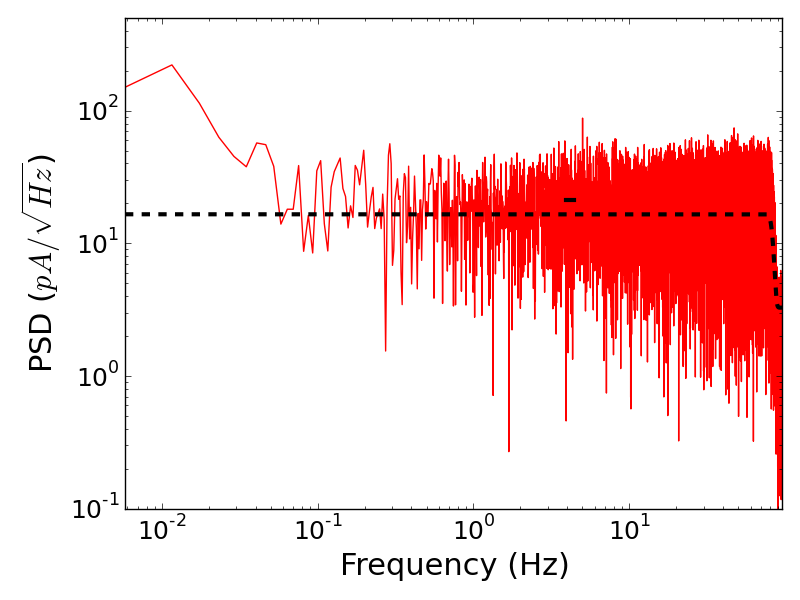
\includegraphics[width=0.48\columnwidth]{figures/board66_wire1_ch03_1356968507s_overbias}
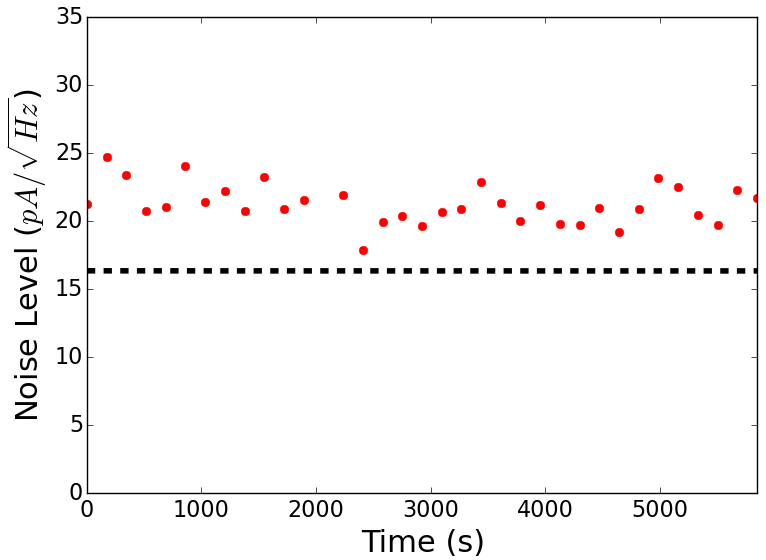
\includegraphics[width=0.48\columnwidth]{figures/board66_wire1_ch03_overbias}
\caption[Spectral density and noise as a function of time for one overbiased bolometer in flight]{Left: the current spectral density of one 150 GHz detector during one 172 s section of the flight when it was overbiased (solid red) and the predicted quadrature sum of the Johnson and readout noise (dashed black). We quote noise levels averaged over a narrow band from 3.9 to 4.4 Hz (thick solid black). Right: the measured to predicted readout and Johnson noise ratio as a function of time for the same detector.
\label{fig:one_bolo_overbias_noise} }
\end{center}
\end{figure}

%IF YOU HAVE TIME, COME BACK AND RELABEL THIS PLOT AS SPECTRAL DENSITY
%ALSO, DO WHAT FRANKY DID AND BIN THE PSD SO IT'S NOT SO FOREST-Y

\begin{figure}[htp]
\begin{center}
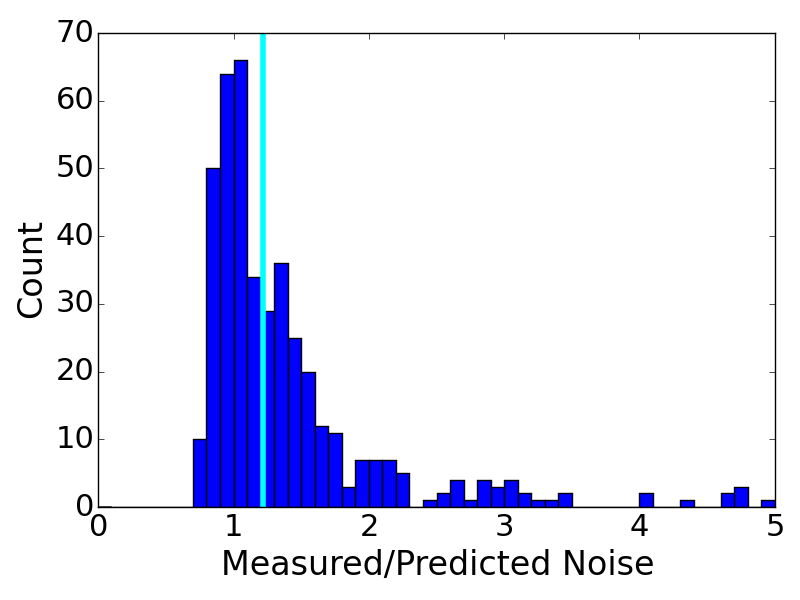
\includegraphics[height=2.5in]{figures/overbias_noise_ratios_histogram}
\caption[In-flight overbiased noise histograms]{Histogram of the median ratio of measured to predicted readout and Johnson noise for all bolometers. 
The prediction for each bolometer has been multiplied by 1.8, the median factor of excess noise measured by the resistor channels. 
There are 34 bolometers with a ratio greater than 5.
The median value (vertical cyan) is 1.2. 
\label{fig:overbias_noise_hist} }
\end{center}
\end{figure}

\begin{table}[htp]
\begin{center}
\begin{tabular}{| c | c | c |}
\hline  
           & Prediction           & Measured   \\
Wafer & (pA/$\sqrt{\mathrm{Hz}}$) & Ratio  \\
\hline 150-09 & 18 &  1.1 \\ 
\hline 150-14 & 17 &  1.1 \\ 
\hline 150-15 & 16 &  1.2 \\ 
%\hline 150-20 & Failed & Failed \\
%\hline 150-24 & 7.0 & 1.57 & Failed \\
\hline 150-39 & 19 &  1.5 \\ 
\hline 150-43 & 19 &  1.1 \\
\hline 150-47 & 21 &  1.1 \\
\hline 250-23 & 19 &  1.0 \\ 
\hline 250-24 & 21 &  1.3 \\ 
%\hline 250-25 & 1.94 & Failed \\
\hline 250-29 & 18 &  1.4 \\
%\hline 410-18 & 5.40 & Failed \\ 
\hline 410-28 & 24 &  1.4 \\
\hline
\end{tabular}
\end{center}
\caption[Median overbiased NEP predictions and measurements for each wafer]{The predicted combination of Johnson and readout noise for each wafer. The theoretical predictions have been boosted by a factor of 1.8, the excess of noise measured by the resistors. For each wafer the measaured to predicted ratio quoted is the median of the distribution for the detectors on that wafer. 
\label{tab:overbias_noise_table} }
\end{table}

%IF YOU HAVE TIME, COME BACK HERE AND INCLUDE OVERBIAS NOISE AS A FUNCTION OF BIAS FREQUENCY!!!!
%IF YOU DON'T UNDERSTAND THIS, WHY ARE YOU INCLUDING IT????

Figure~\ref{fig:overbias_noise_vs_freq} is a plot of the ratio of the overbiased noise prediction to the measurement as a function of the bias frequency. 
Around 1~MHz, we saw a slight but systematic increase in the measured noise. 
This was not understood. 

\begin{figure}[htp]
\begin{center}
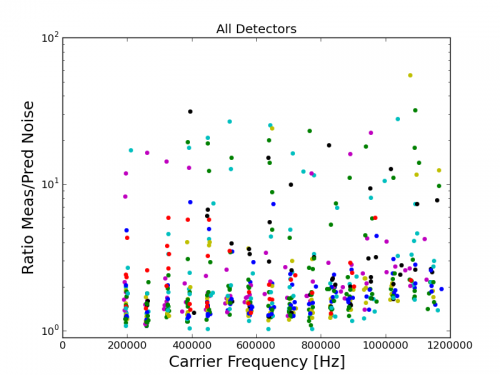
\includegraphics[height=2.5in]{figures/overbias_noise_vs_freq}
\caption[Measured/predicted overbias noise as a function of bias frequency]{Overbias measured to predicted noise ratio as a function of bolometer bias frequency. There is a slight increase in the noise measured for bolometers around a bias frequency of 1~MHz. 
\label{fig:overbias_noise_vs_freq} }
\end{center}
\end{figure}

%IF YOU HAVE TIME, COME BACK AND ADDRESS THIS!!!!
%GROUND MEASUREMENTS IN TX AND MCMURDO
% ALSO, CORRELATION
%Excess overbias noise of roughly the same magnitude was measured when the instrument was on the ground in Antarctica, see \TAB\ref{overbias_noise_table}. 
%The source of the excess overbiased noise is suspected to be electronic. The subset of \ac{EBEX2013} detectors which were present for compatibility testing noise measurements in Palestine, TX, had a median excess overbiased noise a factor of 1.25 greater than predicted. While, at float, this particular subset of detectors had a median overbiased noise factor of 1.58 greater than predicted. Assuming the detectors are overbiased at roughly the same value, they will have comparable temperatures and resistances from run-to-run and there is no physical explanation for an increase in Johnson noise. 
%







%THE FOLLOWING TEXT DOESN'T SEEM TO BE HELPFUL
%In order to isolate the Johnson and readout noise from the phonon and photon noise, we first look at the noise performance with the detectors overbiased. 
%%say when and why we overbias detectors?
%In the normal region of the resistance versus temperature curve, \ac{EBEX} wafer 410-18 detectors have an average slope $dR/dT$ of $0.29\pm0.05 \Omega/K$. 
%At the transition temperature, the average slope of the curve is found to be XXX $\Omega/K$, a factor of XXX greater. 
%The loopgain is proportional to $dR/dT$ and so it is a factor of $\sim XXX$ smaller when the detector is overbiased. 
%The factor $\mathcal{L}/(\mathcal{L}+1)$ is XXX when the detector is normal versus XXX when the detector is overbiased. 
%The dominant noise contributions are then from the Johnson and readout noise. 
%When the detector is overbiased, the current responsivity is low 
%CAN YOU INCLUDE AN UPPER LIMIT OR ESTIMATE?
%and so the dominant noise contributions are from the Johnson and readout noise. 
%But, wait. This quantity is not even \ac{NEP} (it's \ac{NEP}*$S_I$) because the timestream is in A, not W... So what do we call it??)
%These two noise terms are naturally in units of $A/\sqrt{Hz}$ so we can eliminate the uncertainty of the current to power responsivity by comparing the predictions to measurements made in units of $counts/\sqrt{Hz}$ and then converted to current via the demodulated count to Amps \ac{DfMUX} transfer function. 
%We get a handle on the \ac{NEP} contribution of these two terms by comparing the overbiased detector noise prediction to the measurement. 
%The comparison is done in units of $A/\sqrt{Hz}$ so neither the predicted nor the measured results are a function of the detector's current responsivity. 

%The detector white noise level is measured 
%(or is it actually approximated?) 
%by computing the square root of the average value of the \ac{PSD} from 3.9 to 4.4~Hz for a 172~second 
%by computing the average value of the \ac{ASD} from 3.9 to 4.4~Hz for a 172~second 
%(do we write s or second?) 
%timestream, Fig.~\ref{fig:one_bolo_overbias_noise}. 
%Though the \ac{HWP} is not spinning during these overbiased noise measurements, this particular frequency range is chosen to fall in the polarization band, between \ac{HWP} harmonics. 
%to ensure there is no residual \ac{HWP} template biasing the noise measurement. 
%We measure and predict the overbiased noise
%\ac{NEP}(except it is not actually NEP since the bolo is overbiased) 
% noise equivalent current ???

%We then histogram the median measured to predicted overbiased noise ratio of each detector on a wafer in order to quantify the noise performance by wafer, see Fig.~\ref{fig:250-23_overbias_hist} for the histogram of wafer 250-23. 
%are you going to comment on why it's reasonable to take the median ratio? is it actually reasonable?? also, why do this on a wafer-by-wafer basis? do you have evidence that different wafers ought to be treated differently??
%We do this process for each bolometer and then histogram each detector's median ratio of measured to predicted noise, see Fig.~\ref{fig:250-23_overbias_hist} for the results of wafer 250-23. 
%We report each wafer's median measured to predicted overbiased noise in \TAB\ref{overbias_noise_table}. 
%The combination of measured Johnson and readout noise is higher than predicted, where the median value of the excess for all detectors across all observation frequency bands is a factor of 1.7.  

%%%%%%%%%%%%%%%%%%%%%%%%%%%%%%%%%%%%%%%%%%%%%%%%%%%%%%%%%%%%%%%%%%%%%%%%%%%%%%%%
\subsection{In-Flight In-Transition Noise Prediction}
\label{sec:in_trans_pred}
%%%%%%%%%%%%%%%%%%%%%%%%%%%%%%%%%%%%%%%%%%%%%%%%%%%%%%%%%%%%%%%%%%%%%%%%%%%%%%%%

We predicted the in-transition \ac{NEP} in $aW/\sqrt{Hz}$ at the detector. 
The in-transition noise included the readout, Johnson, phonon, and photon noise, Equation~\ref{eq:nep}. 
In order to report the data in units of power at the detector, the readout and Johnson noise, as well as the measured counts from the detector timestream, were divided by the bolometer current responsivity, see Table~\ref{tab:psd_table} for unit conversions. 
We assumed we were in the high loopgain regime so $S_I \sim \sqrt{2}/V_{bias}$. 

The phonon \ac{NEP} contribution was estimated assuming the detector temperature was $T_{c}$ and calculating the thermal conductance as described in Equation~\ref{eq:gbar_to_g}. 
In order to estimate the photon \ac{NEP} contribution at float, we took $P_{rad}$ to be the radiative load measured by each detector, Section~\ref{sec:radiative_load}. 
%These numbers were from franky's code
%The center and width of the observation frequency bands, $\nu$ (155, 256, and 395~GHz) and $\Delta \nu$ (30, 44, and 58~GHz), were from calibration measurements of the \ac{EBEX} spectral response on the ground \cite{Zilic2014}. 
%there numbers were from kyle's thesis
The center and width of the observation frequency bands, $\nu$ (153, 244, and 393~GHz) and $\Delta \nu$ (25, 28, and 45~GHz), were from calibration measurements of the \ac{EBEX} spectral response on the ground \cite{Zilic2014}. 
We did not have a measure of the photon correlation noise factor, so we assumed it was completely correlated, $\xi=1$.
This put an upper bound on the noise prediction and had the greatest effect on the 150~GHz \ac{NEP} prediction. 
%Table~\ref{tab:photon_noise} gives the relative contributions of the correlation and shot noise for the average measured radiative load per observation frequency band.
For the 150~GHz band, if the photons were completely uncorrelated, $\xi=0$, then the photon \ac{NEP} in $W/\sqrt{Hz}$ would have decreased by a factor of 0.80, decreasing the total \ac{NEP} prediction by a factor of 0.90. 
For the 410~GHz band, the decrease in photon \ac{NEP} would have been a factor of 0.95, decreasing the total \ac{NEP} prediction by a factor of 0.98. 
%In reality, the photon noise correlation factor is probably somewhere in between 0 and 1 \cite{}. 


%THESE NUMBERS ARE, SADLY, NOT MAKING SENSE RIGHT NOW. 
%MUST MOVE ON.
%COME BACK IF YOU HAVE TIME.
%\begin{table}[htp]
%\begin{center}
%\begin{tabular}{|c|c|c|c|}
%\hline  
%Band Center & Band Width & Shot NEP & Correlation NEP \\
%(GHz) & (GHz) & (aW^2/Hz$) & (aW^2/Hz$) \\
%\hline 155 & 30 & 740 & 430 \\
%\hline 256 & 57 & 1800 & 490 \\
%\hline 395 & 58 & 2600 & 410 \\
%\hline
%\end{tabular}
%\end{center}
%\caption[Photon shot and correlation noise contributions]{The photon shot and correlation noise contributions as a function of observation frequency band.
%\label{tab:photon_noise} }
%\end{table}
%
%except kyle had 
%nu=153 and dnu = 25
%244, 28
%393, 45


Figure~\ref{fig:prediction_bar_chart} is a stacked bar chart of the \ac{EBEX} in-transition noise prediction per wafer in units of aW/$\sqrt{Hz}$ at the detector. 
Each wafer's bar was the mean for that wafer and the error bars were one standard deviation. 
The blue bar was the predicted \ac{NEP} using the expected radiative load, Table~\ref{tab:target_gbar}, to calculate the photon noise contribution and each detector's carrier and nuller settings as well as its dark characterization measurements to calculate the readout, Johnson, and phonon noise contributions. 
The cyan bar included the additional \ac{NEP} given the \textit{measured} radiative load of each detector. 
The golden bar included the excess factor of 1.8, measured on the resistor channels, applied to the bolometer readout and Johnson noise. 


\begin{figure}[ht!]
\begin{center}
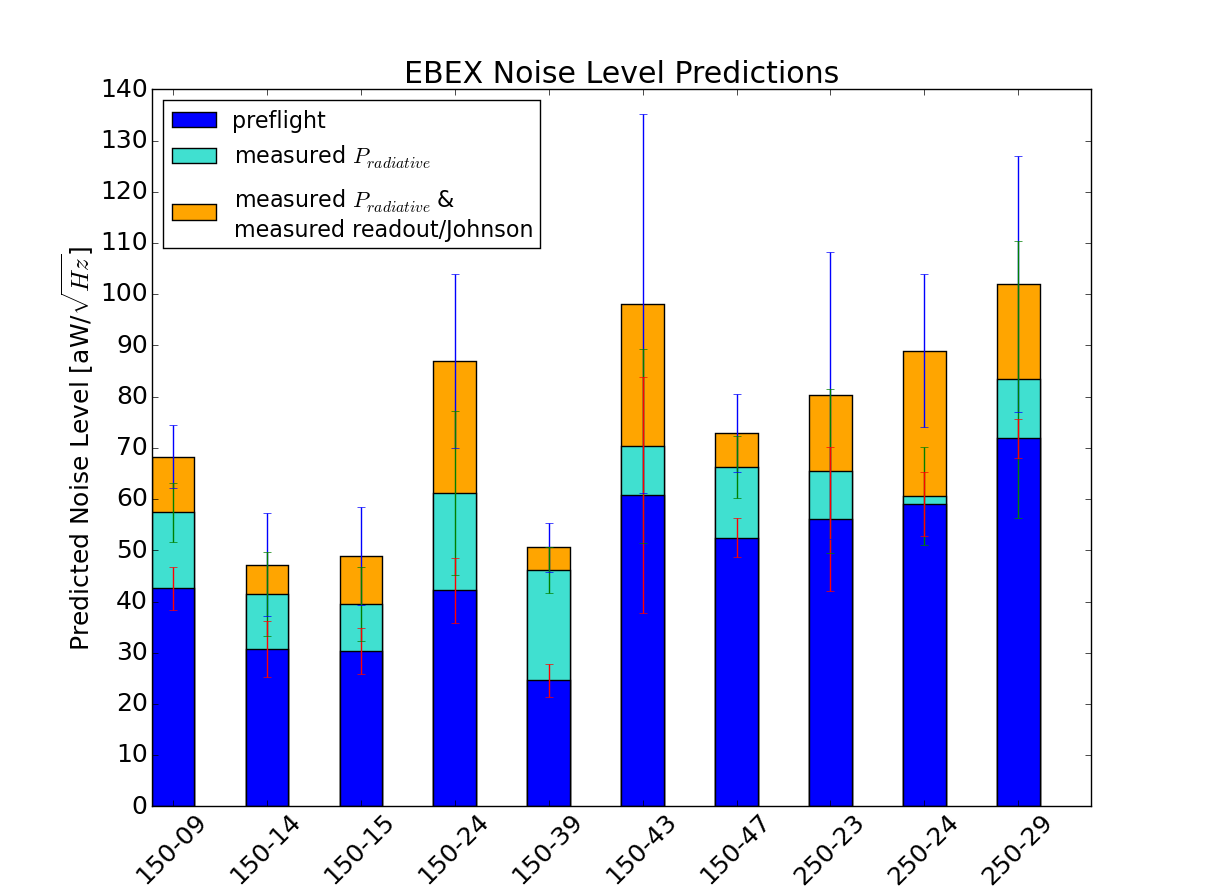
\includegraphics[height=2.5in]{figures/ebex_noise_level_predictions_barchart_per_wafer}
\caption{The \ac{EBEX} pre-flight \ac{NEP} prediction (blue), including the measured radiative load (cyan), and including the boost to readout and Johnson noise (gold).
\label{fig:prediction_bar_chart} }
\end{center}
\end{figure}

Figure~\ref{fig:in_transition_pie} gives the breakdown of the noise components per observation frequency band as pie charts in units of $aW^2/Hz$.
\textcolor{red}{Describe pie charts.}
\textcolor{red}{Remake pie charts as in EP2. make excess a different slice. understand why numbers don't agree!!!}
The median predicted in transition \ac{NEP} level broken down by wafer is reported in \TAB\ref{in_transition_noise_table}. 

% THESE ARE SO DIFFERENT THAN THE PAPER ONES. EVEN/ESPECIALLY PHOTON NOISE. WHY?? 
% REMAKE????
\begin{figure}[ht!]
  \begin{center}
    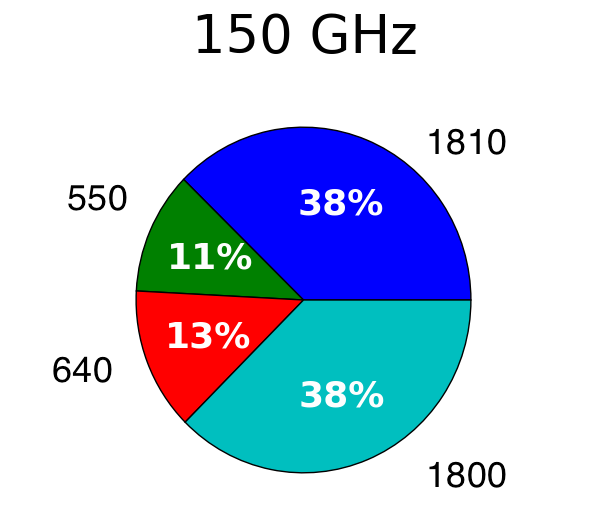
\includegraphics[width=0.29\columnwidth]{figures/150_average_noise_contribution_pie_chart.png}
    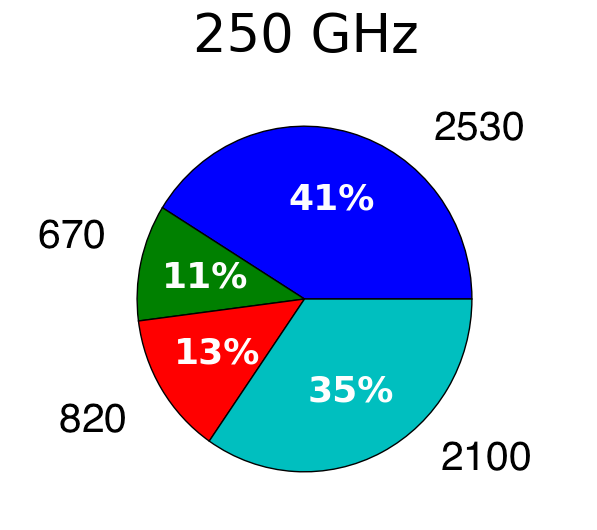
\includegraphics[width=0.29\columnwidth]{figures/250_average_noise_contribution_pie_chart.png}
    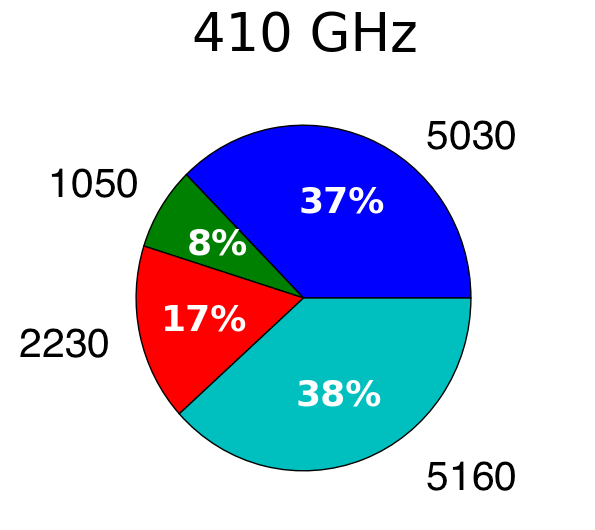
\includegraphics[width=0.29\columnwidth]{figures/410_average_noise_contribution_pie_chart.png}
    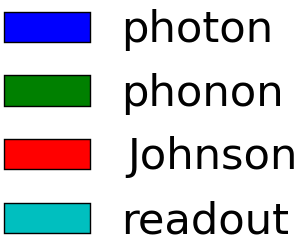
\includegraphics[width=0.1\columnwidth]{figures/piechart_legend.png}
    \caption[In transition noise contributors for each observation frequency band]{Individual components of the \ac{NEP} prediction in aW$^{2}$/Hz per band.
      The readout and Johnson \ac{NEP} terms include the excess factor of 1.8 measured with the resistor channels and with the detectors overbiased.
      % We hypothesize that the excess readout noise is due to electromagnetic pickup.
      \label{fig:in_transition_pie} }
  \end{center}
\end{figure}






%There is a piechart breakdown of each contributor to the predicted \ac{NEP} for one 150~GHz detector towards the beginning of flight in Fig.~\ref{fig:in_transition_psd}. 

%We calculate the theoretical Johnson and readout current noise as described above except we also take into account the factor of excess noise measured with the detector overbiased. 
%We assume the factor of excess remains constant when the detector is in its transition, and for each detector on a wafer, we multiply that detector's theoretical Johnson and readout noise by its wafer's median ratio of overbiased to predicted noise reported in \TAB\ref{overbias_noise_table}. 
%In order to convert from current noise to \ac{NEP} at the detector, we divide the Johnson and readout noise terms by the current responsivity. 
%
%The current responsivity is the current response of the bolometer to incident power,
%\begin{equation}
%S_I = -\frac{dI}{dP} = \frac{-\sqrt{2}}{V_{bias}} * \frac{\mathcal{L}}{\mathcal{L} + 1} * \frac{1}{1 + i\omega\tau}
%\label{eq:current_responsivity}
%\end{equation}
%where $V_{bias}$ is the voltage bias across the bolometer, $\mathcal{L}$ is the bolometer loopgain, $\omega$ is the angular frequency of the signal modulation, and $\tau$ is the bolometer time constant~\cite{Francois2012}. we need to explain and/or reference why dfmux puts a $\sqrt{2}$ in the responsivity.
%Assuming the loopgain, $\mathcal{L}$, is high and the time constant factor can be neglected, the current responsivity simplifies to $-\sqrt{2}/V_{bias}$, where $V_{bias}$ is calculated from the \ac{DfMUX} board settings and the transfer function from bias amplitude to voltage across the \ac{TES}. 
%This analysis assumes the loopgain for each detector is high and we address this assumption in Section XXX. 

%The average thermal conductance has less uncertainty than the dynamic thermal conductance because the measurement of the average thermal conductance does not require knowledge of the power of the thermal conductivity. 
%THIS IS ALREADY DESCRIBED IN THE SECTION ON G
%Though the phonon \ac{NEP} calculation requires knowledge of the dynamic thermal conductance, the dark characterization measurements performed provide only a measure of the average thermal conductance. 
%In order to get from average to dynamic thermal conductance, we assume the thermal conductivity can be described by a power law of power n, $\kappa = \kappa_{0} T^{n}$.
%We then find the dynamic thermal conductance via the following relation between average and dynamic thermal conductance
%\begin{equation}
%G_{dynamic} = (n+1) \frac{1 - T_{bath}/T_{critical}}{1 - T_{bath}^{n+1}/T_{critical}^{n+1}} \times \overline{G}
%\end{equation}
%where $T_{bath}$ is the temperature of the bath, $T_{critical}$ is the detector's measured critical temperature, and n is the power of the thermal conductivity \cite{Mather1982}. 
%In order to calculate $\gamma$, the factor accounting for the temperature gradient along the weak link from the TES to the bath, we again need to assume the thermal conductivity takes the form of a power law of power n. 
%Gamma is then
%\begin{equation}
%\gamma = \frac{(n+1)}{(n+2)} \frac{1 - (T_{bath}/T_{critical})^{n+2}}{1 - (T_{bath}/T_{critical})^{n+1}}
%\end{equation}
%where $T_{bath}$ is the temperature of the bath, $T_{critical}$ is the detector's measured critical temperature, and n is the power of the thermal conductivity \cite{Mather1982}. 
%%\comred{I used the derivations/equations from Hannes' thesis, but he says he follows Mather. Should I cite both of them?}
%$T_{bath}$ is measured by a temperature sensor mounted to the stage and $T_{critical}$ is found during the critical transition temperature measurements.
%We take n to be 2 since thermal conductivity measurements of \ac{EBEX} test flight wafers gave values of 2.2 $\pm$ 0.3, 1.9 $\pm$ 0.2, and 2.1 $\pm$ 0.2 for the 150, 250, and 410 GHz bands respectively \cite{Hubmayr2009}.
%




%%%%%%%%%%%%%%%%%%%%%%%%%%%%%%%%%%%%%%%%%%%%%%%%%%%%%%%%%%%%%%%%%%%%%%%%%%%%%%%%
\subsection{In-Flight In-Transition Noise Measurement}
\label{sec:in_trans_meas}
%%%%%%%%%%%%%%%%%%%%%%%%%%%%%%%%%%%%%%%%%%%%%%%%%%%%%%%%%%%%%%%%%%%%%%%%%%%%%%%%


The \ac{HWP} was spinning during the in-transition noise measurements. 
There was a large \ac{HWP} synchronous signal in the raw timestream which had to be subtracted in order to extract the \ac{WNL}. 
Figure~\ref{fig:in_transition_psd} is the square root of the \ac{PSD} of a 172~second chunk of time with the \ac{HWP} synchronous signal present (red) and subtracted (gold) for a detector on wafer~150-09. 
%there was an additional step in the noise analysis pipeline. 
 %of removing the \ac{HWP} synchronous signal from the timestream. 
Just as for the other noise measurements, the measured \ac{WNL}, indicated by the short thick black line, was the square root of the average of the \ac{PSD} between 3.9 and 4.4~Hz. 
The \ac{NEP} prediction, indicated by the thin black dashed line, was calculated as described in Section~\ref{sec:in_trans_pred}. 

\begin{figure}[htp]
\begin{center}
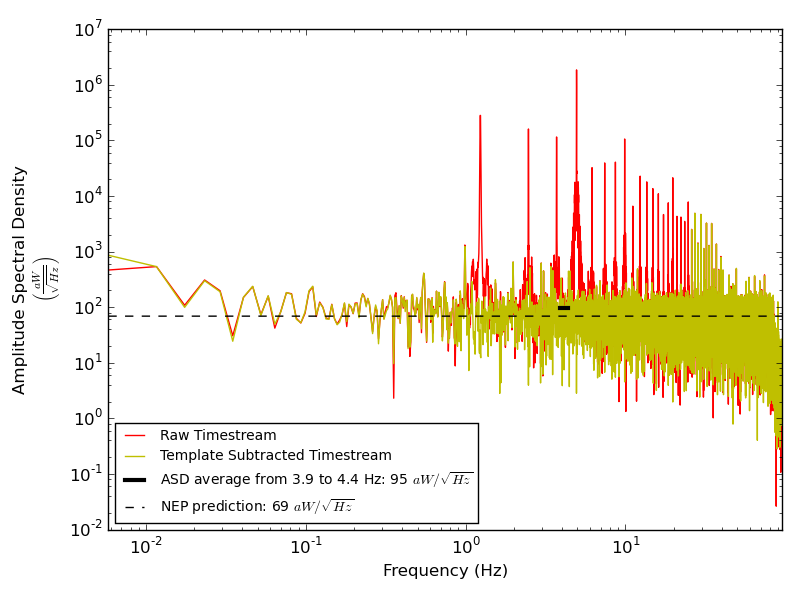
\includegraphics[height=4in]{figures/board68_wire2_ch04_1356979731s_transition.png}
\caption[In-transition spectral density with and without HWP synchronous signal]{In-transition noise with the \ac{HWP} template present (red) and subtracted (gold).
\label{fig:in_transition_psd} }
\end{center}
\end{figure}
%IF YOU HAVE TIME, REMAKE THIS PLOT WITH LARGER LABELS!

%Perhaps, if you want, you can include the flow charts describing how we removed the hwpss ?
%The white noise level is measured exactly as is done in the case of overbiased noise, except the timestream has had the \ac{HWP} template subtracted. 

%YOU DON'T SAY WHAT OBSERVATIONS ARE!
%For approximately ten minutes after the detectors were tuned for Observation C, the \ac{HWP} was off. 
For approximately ten minutes towards the beginning of flight, the detectors were tuned and the \ac{HWP} was off. 
Figure~\ref{fig:hwp_on_vs_off} compares the median \ac{WNL} during the ten minutes with the \ac{HWP} stationary to the median \ac{WNL} during the ten minutes after the \ac{HWP} was turned on. 
%The only difference should have been the subtraction of the HWPSS from the raw timestream while the hwp was spinning. oh, and that the hwp was spinning.   time, with the \ac{HWP} spinning and the template subtracted timestream data, . 
%We expected there to be no difference. 
There was an average increase of XXX when measuring the \ac{NEP} of the template subtracted data versus that measured from the "raw" timestream when the \ac{HWP} is still. 
The subtraction of the \ac{HWP} synchronous signal should not have increased the noise level of the timestream, so we suspect something about the \ac{HWP} increased the measured \ac{NEP}. 

\begin{figure}[ht!]
\begin{center}
%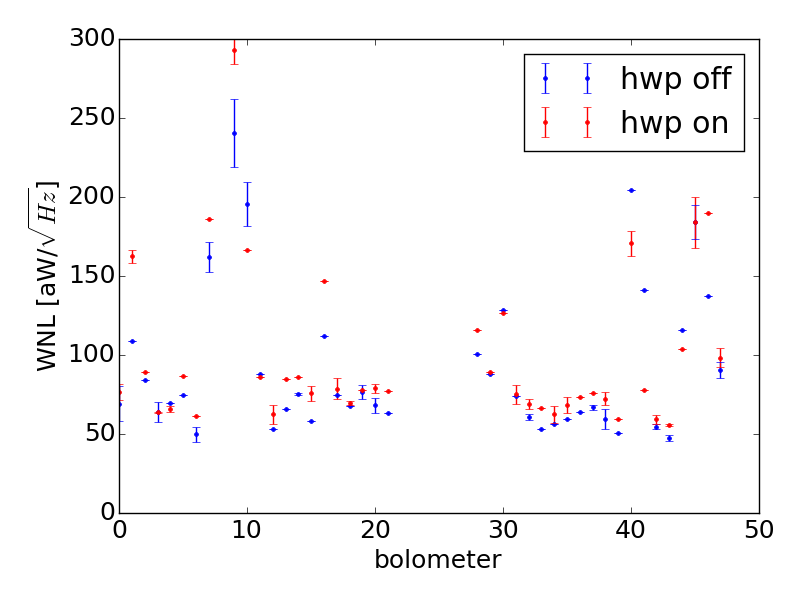
\includegraphics[width=0.4\columnwidth]{figures/hwp_on_and_off_cutoff_at_300aW.png}
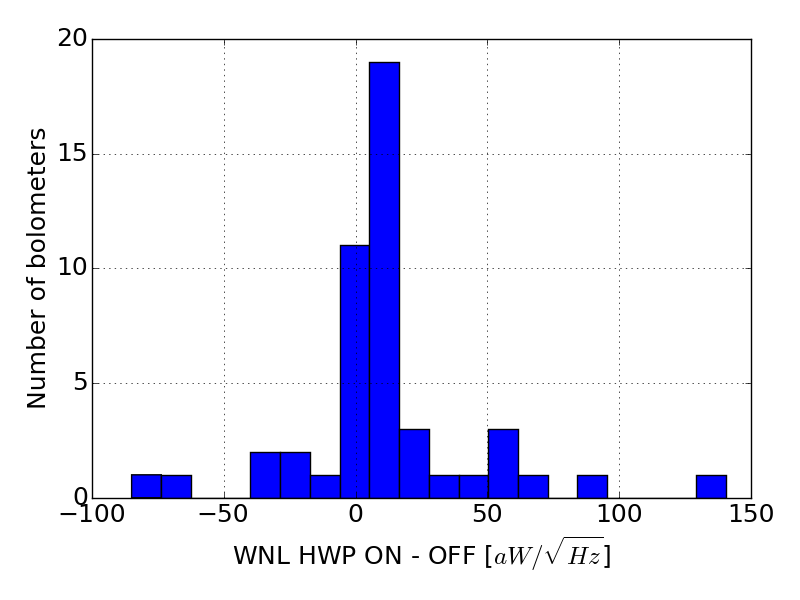
\includegraphics[height=2.5in]{figures/hwp_on_and_off_median_diff_histogram.png}
\caption[Histogram of difference between noise measured with the HWP on and off]{Histogram of the difference between the median \ac{NEP} measured with the \ac{HWP} on and off. 
\label{fig:hwp_on_vs_off} }
\end{center}
\end{figure}



For those detectors which have all of the dark measurements available, throughout flight the noise is calculated and predicted every 172 seconds, provided none of the bolometer timestream data in that chunk has been flagged as bad. 
The noise, measured and predicted, as a function of time is shown for 150-09-XX-XX in Fig.~\ref{fig:in_transition_noise_vs_time}. 
%The median value of the ratio of measured to predicted \ac{NEP} for each detector throughout flight is found. 
The histogram of the median measured to predicted \ac{NEP} for each detector on wafer 150-09 is shown in Fig.~\ref{fig:150-09_median_histogram}.
Each wafer's median measured to predicted \ac{NEP} ratio is reported \TAB\ref{in_transition_noise_table}. 
Taking into account the excess overbiased noise and using each detector's measured radiative load, the measured \ac{NEP} agrees with the predictions to within one standard deviation. 





\begin{figure}[ht!]
\begin{center}
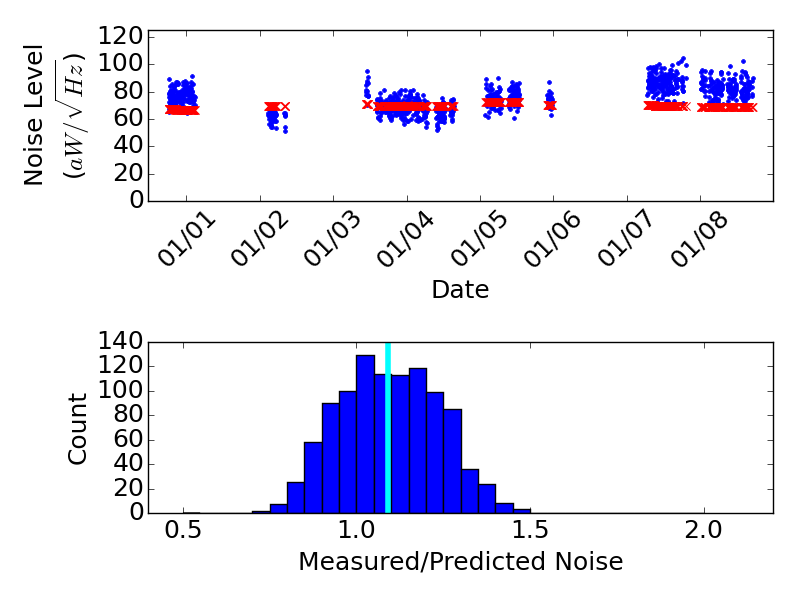
\includegraphics[width=0.48\columnwidth]{figures/board68_wire2_ch06_transition.png}
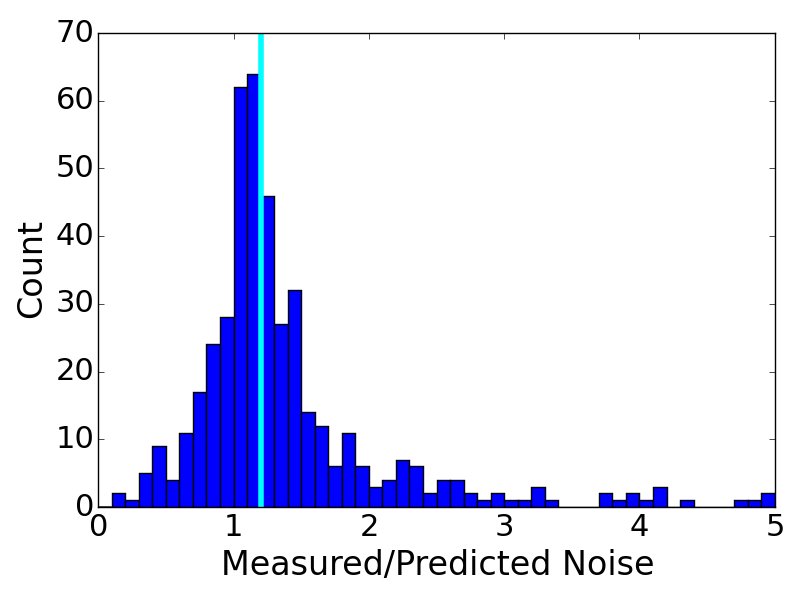
\includegraphics[width=0.48\columnwidth]{figures/in_transition_histogram.png}
\caption{Left top: in-transition measured (blue dots) and predicted corrected for excess noise above the transition (red crosses) \ac{NEP} for one 150~GHz detector 
throughout flight. Gaps indicate times that data is absent or rejected. 
Left bottom: distribution 
of measured-to-predicted ratio for this detector throughout flight, and the median (vertical cyan) ratio of 1.1.
Right: the distribution of the median ratio of measured to predicted in-transition noise corrected for excess noise above the transition throughout flight for all bolometers.
The median ratio (vertical cyan) is 1.2. 
\label{fig:in_transition_noise} }
\end{center}
\end{figure}



\begin{table}[ht!]
\begin{center}
\begin{tabular}{|c|c|c|c|}
\hline  Wafer & Predicted NEP [aW/$\sqrt{\mathrm{Hz}}$] & Measured/Predicted NEP \\
\hline 150-09 & 68 & 1.1 \\
\hline 150-14 & 45 & 0.8 \\
\hline 150-15 & 47 & 1.2 \\
%\hline 150-20 & n/a \\
%\hline 150-24 & n/a \\
\hline 150-39 & 77 & 1.1 \\
\hline 150-43 & 56 & 1.1 \\
\hline 150-47 & 59 & 1.4 \\
\hline 250-23 & 80 & 1.1 \\
\hline 250-24 & 76 & 1.4 \\
%\hline 250-25 & n/a \\
\hline 250-29 & 93 & 1.5 \\
%\hline 410-18 & n/a \\
\hline 
410-28 & 110 & 1.6 \\
\hline
All Detectors &  & 1.2 \\
\hline
\end{tabular}
\end{center}
\caption{The median predicted \ac{NEP} and measured-to-predicted ratio corrected for excess noise above the superconducting transition for each wafer and combined for 
all detectors.
}
\label{tab:in_transition_noise_table}
\end{table}






%%%%%%%%%%%%%%%%%%%%%%%%%%%%%%%%%%%%%%%%%%%%%%%%%%%%%%%%%%%%%%%%%%%%%%%%%%%%%%%%
\subsection{Loopgain}
\label{sec:loopgain}
%%%%%%%%%%%%%%%%%%%%%%%%%%%%%%%%%%%%%%%%%%%%%%%%%%%%%%%%%%%%%%%%%%%%%%%%%%%%%%%%

In order to convert from units of current to power at the detector, these results assume the detectors are operating deep in their transitions. 
A detector well into its transition has a high loopgain and so $\mathcal{L}/(\mathcal{L} + 1) \sim 1$, and the current responsivity can be approximated as $-\sqrt{2}/V_{bias}$. 
If, however, the detector is not dropped deep into its transition, then it is not safe to assume the loopgain is high and the factor of  $\mathcal{L}/(\mathcal{L} + 1)$ in the responsivity should not be neglected. 
%The \ac{EBEX} detectors are dropped to 85\% of their normal resistance for the majority of flight. 
We can estimate the loopgain at any depth in the transition via the definition of loopgain, 
\begin{equation}
\mathcal{L} \equiv \frac{P\alpha}{GT}
\end{equation}
where $P$ is the Joule power dissipated in the bolometer, alpha is a unitless number quantifying the temperature sensitivity, $G$ is the dynamic thermal conductance, and $T$ is the bolometer temperature \cite{Enss2005}. 
The largest uncertainty is in the value of $\alpha$, 
 \begin{equation}
 \alpha \equiv \frac{\partial \log R}{\partial \log T}=\frac{T}{R} \frac{dR}{dT}
 \end{equation}
 where R is the detector resistance and T is the detector temperature \cite{Enss2005}. 
The \ac{EBEX} detector resistances are known to 10\%, but near the transition, $dR/dT$ changes steeply given small changes in detector resistance. 
If we take a typical resistance versus temperature curve and overestimate the average value of R by 10\%, then $\mathcal{L}$ decreases by a factor of 2.
If we underestimate R by 10\%, then $\mathcal{L}$ increases by a factor of 7. 
%\comred{Provide a quantitative uncertainty on $\alpha$ given the uncertainty on R \& dR/dT.}
Given this, can we even report on/conclude anything from the loopgain measurements??

In order to provide an estimate of the effect of operating the detectors at 85\%, near the top of their transitions, we calculate the loopgain for the detectors on wafer 250-23. 
The left panel of Fig.~\ref{fig:loopgain_histogram} is a histogram of the calculated loopgains for one tuning of these detectors during flight. 
When we perform the analysis of the noise performance using the measured loopgains instead of assuming the loopgain is 10000, we find the ratios of measured to predicted noise in the right panel of Fig.~\ref{fig:loopgain_histogram}. 
The median ratio increases from 1.05 to 1.15. 
Our final results reported in \TAB\ref{in_transition_noise_table} are a lower limit on the noise performance, and if all wafers behave similarly to wafer~250-23, taking into account the measured loopgain increases the ratio of measured to predicted noise by $\sim$10\%. 


 %\comred{is referencing the irwin/hilton chapter the right thing to do?}
%If the resistance values are systematically 10\% too low, then the median loopgain changes from 9 to 7. 
%If instead the resistance values are systematically 10\% too high, then the median loopgain changes from 9 to 20. 

% would like to include iv curve loopgains as well, BUT I still don't understand how the equation follows from the referenced paper in ziggy's thesis.
%The loopgain can also be estimated from the iv measurement. 
%\comred{You need to comment on how safe (or un-safe) it is to make those sweeping assumptions that loopgain is huge and time constant correction factor is neglect-able}
% do we say in transition or in-transition ? 

\begin{figure}[ht!]
\begin{center}
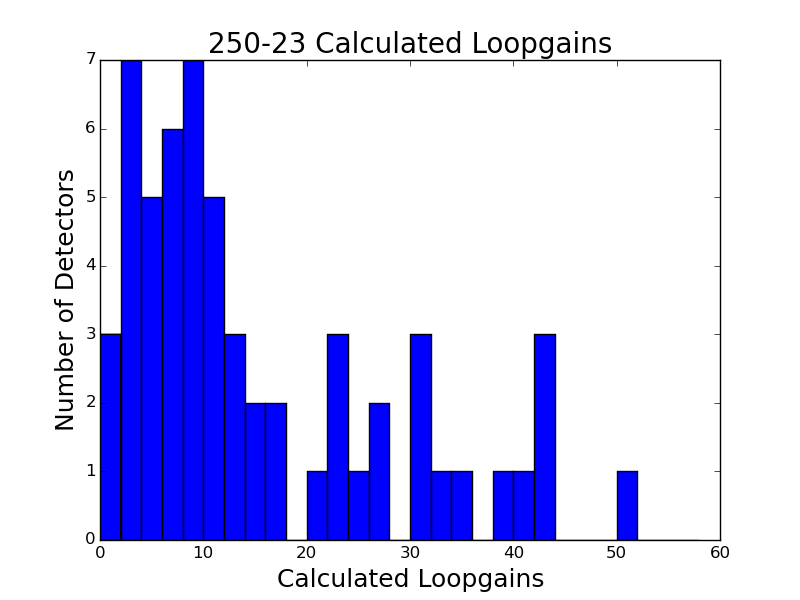
\includegraphics[width=0.4\columnwidth]{figures/250-23_calculated_loopgains_histogram.png}
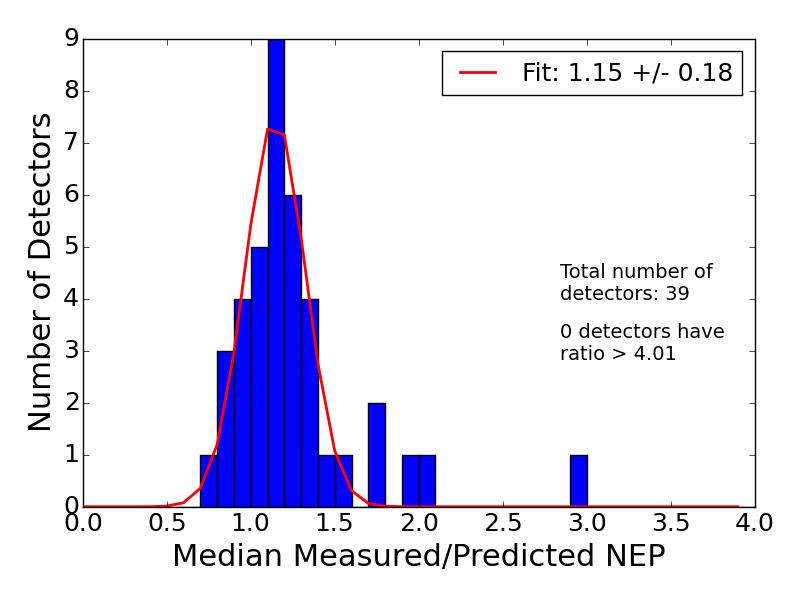
\includegraphics[width=0.4\columnwidth]{figures/250-23_meas_pred_ratios_obsc_calculated_loopgain.png}
\caption{{\it Left:} The calculated loopgains for wafer 250-23 using Joule power measured from flight iv curves, alpha and temperature from dark resistance versus temperature measurements, and thermal conductance from dark iv curves and assuming the power of thermal conductivity is 2. {\it Right:} The median ratio of measured to predicted \ac{NEP} for each detector on wafer 250-23 using the calculated loopgains instead of assuming the detector is deep in its transition and the loopgain is 10000.}
\label{fig:loopgain_histogram}
\end{center}
\end{figure}


\begin{figure}[htbp]
\begin{center}
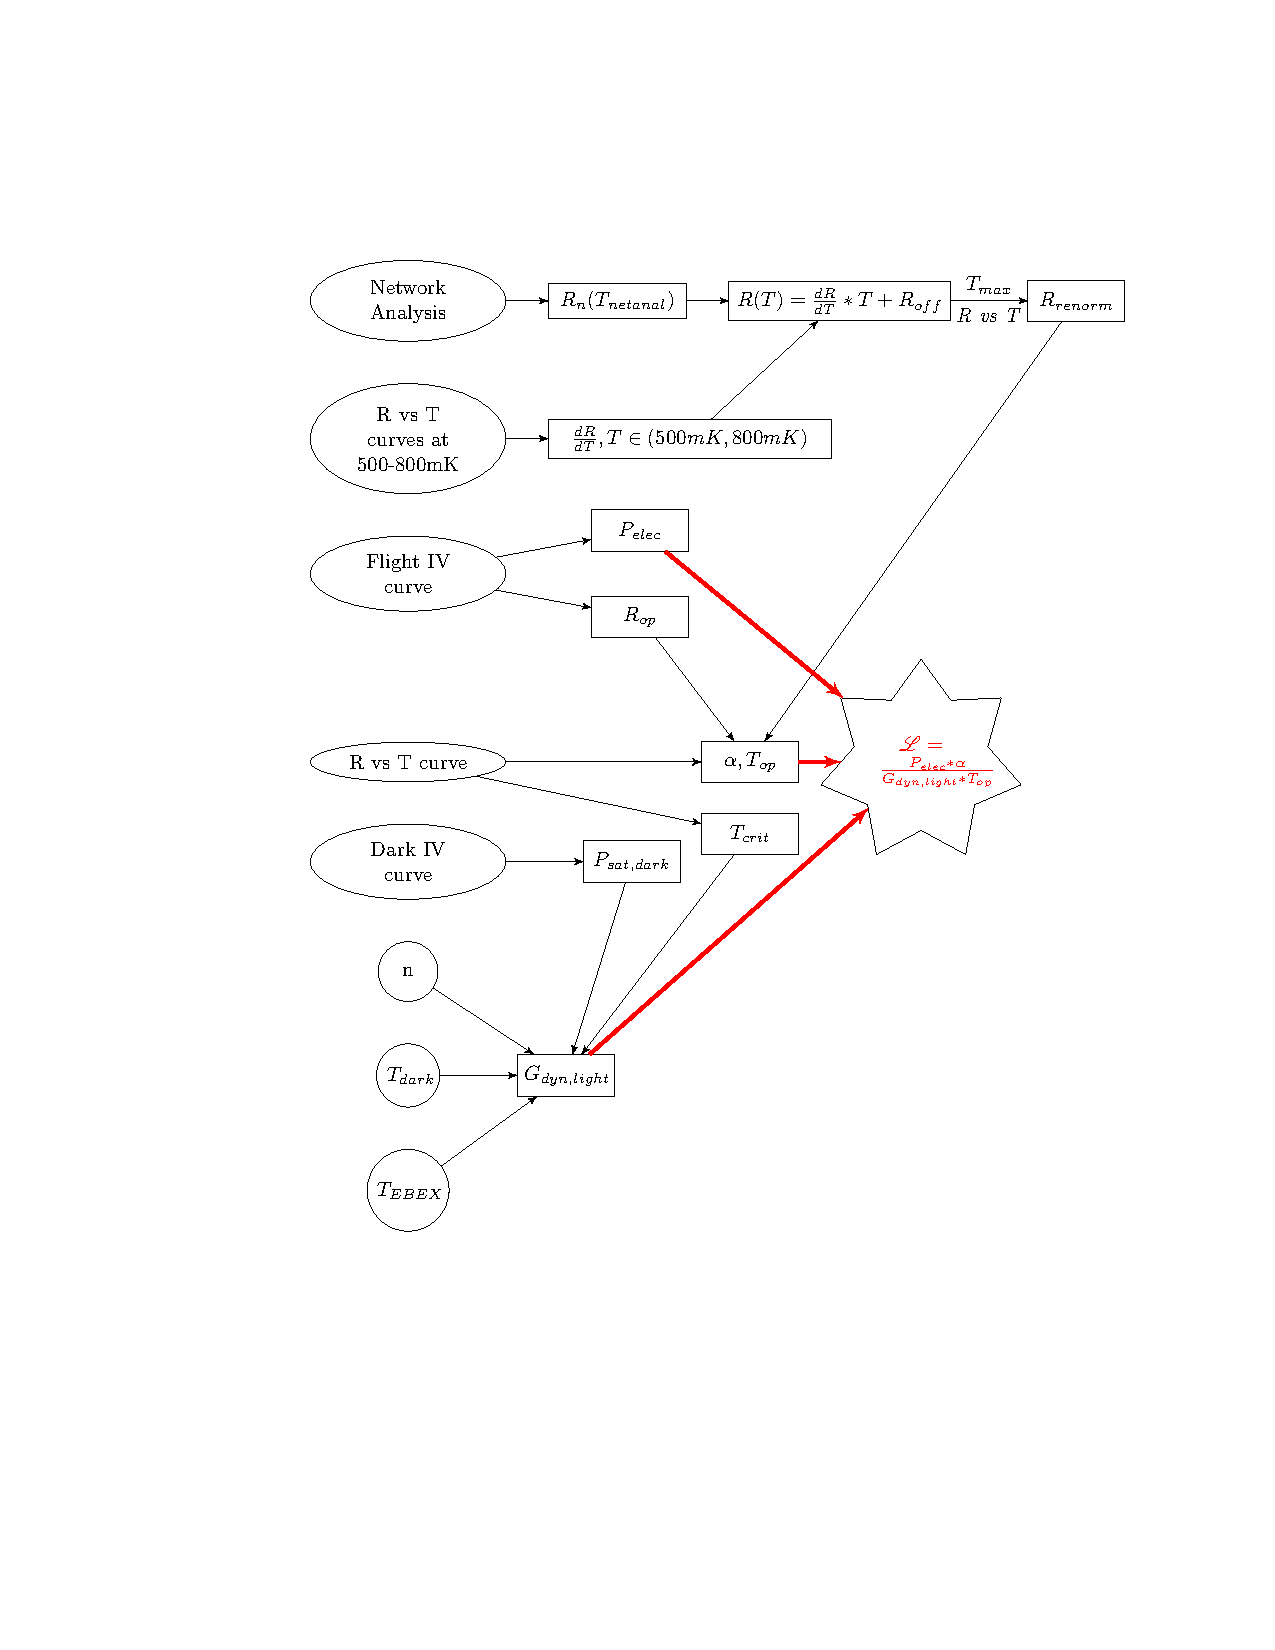
\includegraphics[width=1.0 \textwidth]{figures/loopgain_flowchart.pdf}
\caption{Loop gain calculation flow chart}
\label{fig:loopgain_flow}
\end{center}
\end{figure}

The slope of the Resistance vs Temperature curve for 410-18 between .550 and .800~K was $0.29\pm0.05 \Omega/K$. 

\begin{figure}[htbp]
\begin{center}
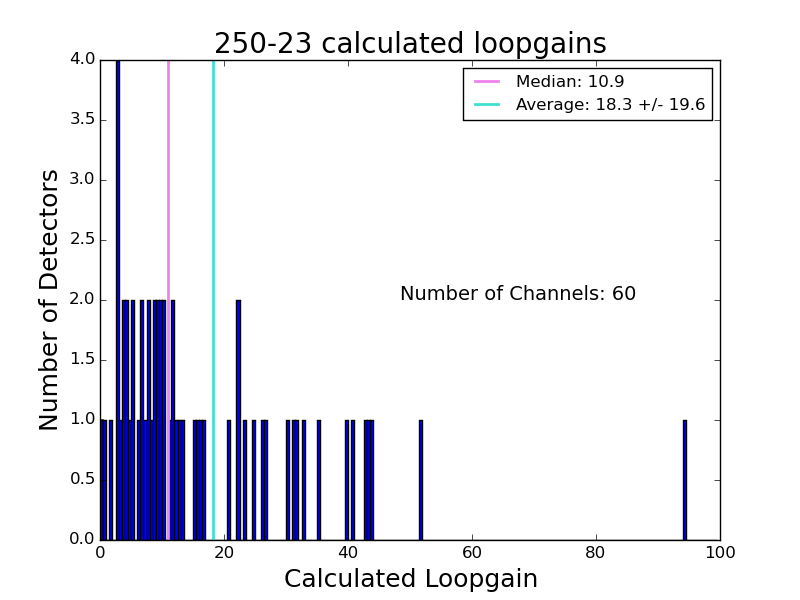
\includegraphics[width=0.5 \textwidth]{figures/250-23_loopgains_calculated_tuning3.png}
\caption{Loop gains calculated for 250-23 for tuning3.}
\label{fig:loopgain_calc_hist}
\end{center}
\end{figure}

\begin{figure}[htbp]
\begin{center}
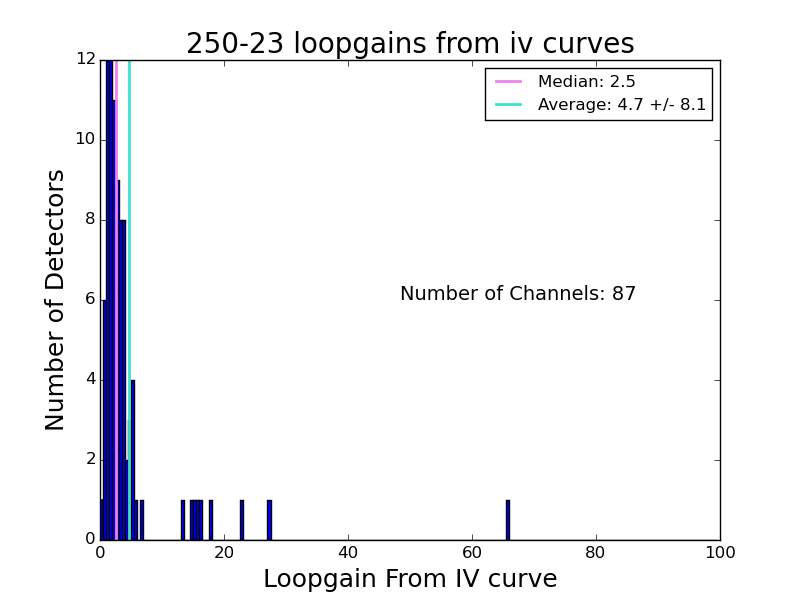
\includegraphics[width=0.5 \textwidth]{figures/250-23_loopgains_from_iv_tuning3.png}
\caption{Loop gains estimated from each 250-23 bolometer's flight IV curve for tuning3.}
\label{fig:loopgain_from_iv_hist}
\end{center}
\end{figure}

%%%%%%%%%%%%%%%%%%%%%%%%%%%%%%%%%%%%%%%%%%%%%%%%%%%%%%%%%%%%%%%%%%%%%%%%%%%%%%}}}

